% Created 2024-09-25 Wed 00:53
% Intended LaTeX compiler: xelatex
\documentclass[letterpaper]{article}
\usepackage{graphicx}
\usepackage{longtable}
\usepackage{wrapfig}
\usepackage{rotating}
\usepackage[normalem]{ulem}
\usepackage{capt-of}
\usepackage{hyperref}
\usepackage{fontspec}
\setmainfont[Ligatures=TeX]{CMU Serif}
\usepackage{bookmark}
\usepackage{amssymb}
\usepackage{amsmath}
\setlength{\parindent}{0pt}
\author{Gleb Anohin}
\date{\today}
\title{analysis quantifier}
\hypersetup{
 pdfauthor={Gleb Anohin},
 pdftitle={analysis quantifier},
 pdfkeywords={},
 pdfsubject={},
 pdfcreator={Emacs 29.1 (Org mode 9.8)}, 
 pdflang={English}}
\begin{document}

\maketitle
\tableofcontents

\section{Кванторы и струтктура теорем}
\label{sec:org875b29e}
\(\forall\) -- кватор всеобщности -- для любого

\(\exists\) -- квантор существования -- существует

\(\exists!\) -- квантор единственности -- существует лишь один

\(\forall x: A(x) \rightarrow B(x)\) пишут \(A(x) \rightarrow B(x)\)

Говорят: достаточно для; достаточный признак; необходимое условие для; только тогда, когда; B следует из A; B вытекает из A.

Если \(A(x) \rightarrow B(x)\) и \(B(x) \rightarrow A(x)\), то пишут \(A(x) \iff B(X)\)

Говорят: равносильно, тогда и только тогда
\subsection{Примеры}
\label{sec:org4e0c7de}
\subsubsection{1}
\label{sec:org7072284}
\(A = \{x: P(x)\}, B = \{x: Q(x)\}\)

Доказать: \(P(x) => Q(x) \iff A \subset B\)

\(P(x) \rightarrow Q(x) \iff \forall x: P(x) \rightarrow Q(x)\)

Необходимость: \(x \in A \rightarrow P(x) = T \rightarrow Q(x) = T \rightarrow x \in B\)
Достаточность:
\begin{equation}
\begin{cases}
x \in A \Rightarrow P(x) = T\\
x \in B \Rightarrow Q(x) = T
\end{cases}
\Rightarrow P(x) \rightarrow Q(x)
\end{equation}

\begin{equation}
\begin{cases}
x \in A \Rightarrow P(x) = F \\
\left[
\begin{array}{ll}
x \in B \\
x \notin B
\end{array}
\right.
\iff
\left[
\begin{array}{ll}
Q(x) = T \\
Q(x) = F
\end{array}
\right.
\end{cases}
\end{equation}
что и является определением импликации.
\subsubsection{2}
\label{sec:orgb4eaf1a}
Установить устинностное значение

\begin{equation}
\begin{aligned}
\forall c \exists b \forall x: x^2 + bx + c > 0 \\
\forall c \exists b: D < 0 \\
\forall c \exists b: b^2 - 4c < 0 \\
\forall c \exists b: b^2 < 4c \\
b^2 > 0 \Rightarrow 4c > 0
\end{aligned}
\end{equation}

Но это неправда (например при c = -1), следовательно изначальное утверждение ложное
\subsubsection{3}
\label{sec:orgff8c062}
\((x + y = 1) \land ((x <= 3) \rightarrow (x > y))\)
\((x + y = 1) \land ((x > 3) \lor (x > y))\)

\begin{center}
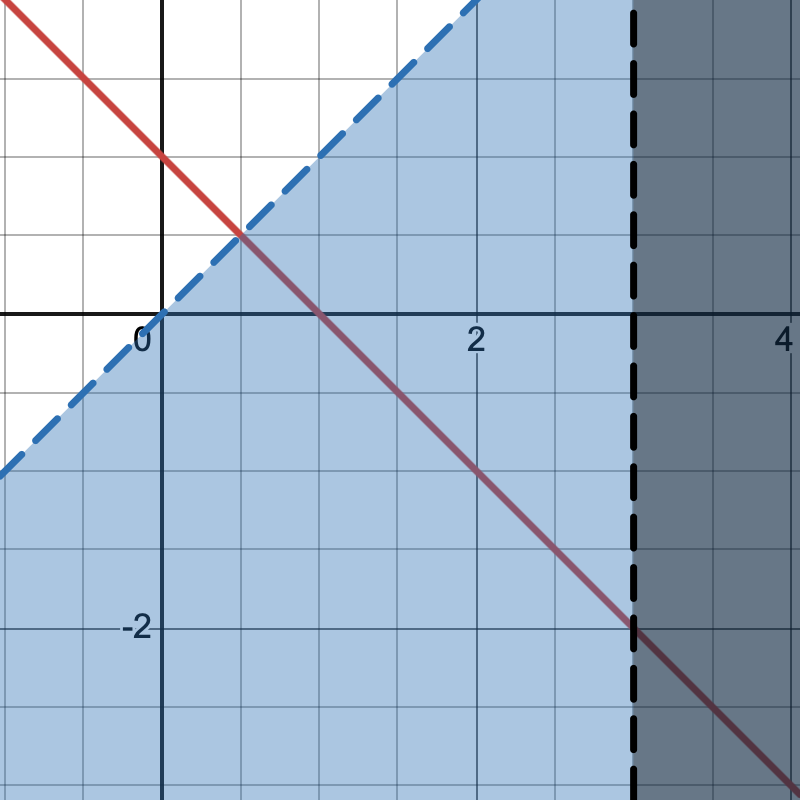
\includegraphics[width=.9\linewidth]{./src/quantifier_graph.png}
\end{center}

Если построить это таким график, то ответом будет та часть прямой, которая находится хотя бы в одном из регионов.

Эту прямую можно упроситить до вида  \(x = 1 - y {x >= 0.5}\)
\subsubsection{4}
\label{sec:org7799f6a}
Построить отрицание к
\(\forall \epsilon > 0 \exists \delta > 0 \forall x_1 \in [0;1] \forall x_2 \in [0;1]: |x_1 - x_2| < \delta \rightarrow |x_1^2 - x_2^2| < \epsilon\)

\(A = \neg{(|x_1 - x_2| < \delta)} \lor |x_1^2 - x_2^2| < \epsilon\)
\end{document}
